\documentclass{article}



% if you need to pass options to natbib, use, e.g.:
%     \PassOptionsToPackage{numbers, compress}{natbib}
% before loading neurips_2022


% ready for submission
\usepackage[preprint]{neurips_2022}


% to compile a preprint version, e.g., for submission to arXiv, add add the
% [preprint] option:
%     \usepackage[preprint]{neurips_2022}


% to compile a camera-ready version, add the [final] option, e.g.:
%     \usepackage[final]{neurips_2022}


% to avoid loading the natbib package, add option nonatbib:
%    \usepackage[nonatbib]{neurips_2022}
\usepackage{mathptmx}
\usepackage{graphicx}
\usepackage{anyfontsize}
\usepackage{t1enc}
\usepackage{amsthm}
\usepackage{amssymb}
\usepackage[utf8]{inputenc} % allow utf-8 input
\usepackage[T1]{fontenc}    % use 8-bit T1 fonts
\usepackage{hyperref}       % hyperlinks
\usepackage{url}            % simple URL typesetting
\usepackage{booktabs}       % professional-quality tables
\usepackage{amsfonts}       % blackboard math symbols
\usepackage{nicefrac}       % compact symbols for 1/2, etc.
\usepackage{microtype}      % microtypography
\usepackage{xcolor}         % colors
\usepackage{amsmath}
\usepackage{hyperref}      % To remove red rectangle around contents
\hypersetup{pdfborder=0 0 0}
\graphicspath{ {./images/} }


\title{Assignment 2}


% The \author macro works with any number of authors. There are two commands
% used to separate the names and addresses of multiple authors: \And and \AND.
%
% Using \And between authors leaves it to LaTeX to determine where to break the
% lines. Using \AND forces a line break at that point. So, if LaTeX puts 3 of 4
% authors names on the first line, and the last on the second line, try using
% \AND instead of \And before the third author name.


\author{%
 % David S.~Hippocampus\thanks{Use footnote for providing further information
   % about author (webpage, alternative address)---\emph{not} for acknowledging
   % funding agencies.} \\
  Indian Institute of Information, Kanpur\\
  Department of Computer Science\\
  CS771 Introduction to Machine Learning\\
  Instructor: Purushottam Kar \\\\ 
  Submitted: November 1, 2022
  %Pittsburgh, PA 15213 \\
  %\texttt{hippo@cs.cranberry-lemon.edu} \\
  % examples of more authors
  \AND
  Ambati Madhav  \\
 160098\\
  % \texttt{email} \\
  \And
  Kudupudi Mohan Kumar \\
  % Affiliation \\
  22105037 \\
  % \texttt{email} \\
   \And
  Abhinav Kuruma \\
  % Affiliation \\
  22111401 \\
 \AND
  % \texttt{email} \\
  Gnanendra Sri Phani Sai Channamsetty \\
  % Affiliation \\
  22105032 \\
  \And
  Rahul Aggarwal\\
 22111403\\
}


\begin{document}
\maketitle


%Sections \ref{gen_inst}, \ref{headings}, and \ref{others} below.
\newpage
\tableofcontents
\newpage
\section{Answer 1}
As we have to map binary digits 0,1 to signs -1,+1,\\
We should make a function say, $m:\{0,1\} \to \{-1,+1\}$. Such that \\
$$
m(x)=\begin{cases}
			-1, & \text{if $x=1$ }\\
            +1, & \text{if $x=0$}\\
	   \end{cases}
$$
and another function named $f:\{-1,+1\} \to \{0,1\}$ and it should be such that \\
$$
f(x)=\begin{cases}
			0, & \text{if $x=+1$ }\\
            1, & \text{if $x=-1$}\\
		 \end{cases}
$$

So, for $m$ the fuction is $m(x) =1 -2x$ and for $f$ the function is $f(x) = \frac{1-sign(x)}{2}$.\\\\
And, we also observe that $f$ is the inverse of $m$. Now, let's take an example to see that
\begin{equation}
XOR(b_1,b_2, \dots ,b_n) = f\left( \prod_{i=1}^n m(b_i) \right)
\end{equation}
\\
Assume $b_1=0,b_2=1,b_3=1$

\begin{equation} \label{eq1}
\begin{split}
XOR(0,1,1) & = f( m(0) * m(1) * m(1) )\\
& = f(1*-1*-1) \hspace{2cm} \text{$\because$} m(x) = 1-2x\\
& = f(1)\\
& = 0  \hspace{4cm} \text {$\because$} f(x) = \frac{1-sign(x)}{2}\\
\end{split}
\end{equation}
\\
Hence, we can implement XOR in this manner.


\section{Answer 2}
\label{gen_inst}
\textbf{(To prove)}  To exploit the above result, first give a mathematical proof that for any real numbers
(that could be positive, negative, zero) \emph{$r_1$, $r_2$, . . . ,$ r_n$} for any n $\in$ N , we always have
\[\prod_{i=1 }^n sign(r_i) = sign \prod_{i=1}^n r_i\]

\paragraph{(Proof)}
To get the sign of a number we can use the following:
\begin{equation} \label{eq2}
sign(r)= \frac{|r|}{r}
\end{equation}
where,
$$
sign(r)=\begin{cases}
			-1, & \text{if $r<0$ }\\
            1, & \text{if $r>0$}\\
	0, & \text{if $r=0$}
		 \end{cases}
$$
Using above definition we can say that,
\[ \frac{|r_1||r_2|...|r_n|}{r_1r_2...r_n} = \frac {|r_1r_2...r_n|}{r_1r_2...r_n}\]
proving this will prove the theorem.\\

\subsection{Case 1}

$ \text{For,} \, r_i \ne 0  \;\, \forall_{i=0}^n r_i $
\begin{equation} \label{eq3}
\begin{split}
\text{ L.H.S } & =  \prod_{i=1 }^n sign(r_1)  \\
& = sign(r_1)*sign(r_2)*\dots *sign(r_n)  \\
& = \frac{|r_1|}{r_1}*\frac{|r_2|}{r_2}*\dots * \frac{|r_n|}{r_n}\\
& = \frac{|r_1||r_2|...|r_n|}{r_1r_2...r_n}\, \hspace{1cm} \text{($\because$ Product term amount to positive value)}\\
\end{split}
\end{equation}
\[sign \, \text{of L.H.S depends on}\, (\frac{1}{r_1r_2...r_n})\]
\\
\begin{equation} \label{eq4}
\begin{split}
\text{ R.H.S } & =  sign \prod_{i=1}^n r_i \\
& = sign[(r_1)*(r_2)*\dots *(r_n)]  \\
& = \frac{|r_1*r_2* \dots *r_n|}{r_1*r_2* \dots *r_n} \hspace{5cm}\\
& = \frac{|r_1r_2\dots r_n|}{r_1r_2...r_n} \hspace{2cm} \text{($\because$ The numerator itself is positive)} \\
\end{split}
\end{equation}

Let $r_1*r_2* \dots *r_n $ = x,\\
Then, we get from equation \ref{eq2}  $\frac{|x|}{x}$, and \\
$$
|x|=\begin{cases}
			-x, & \text{if $x<0$ }\\
            x, & \text{if $x>0$}\\
		 \end{cases}
$$
So, anyways numerator becomes positive. As it is a modular function. So, \\
\[ sign \, \text{of R.H.S depends on} \, (\frac{1}{r_1r_2 \dots r_n}) \hspace{2cm} \]\\\\
\hspace*{6cm}  L.H.S=R.H.S\\ %mkc

\subsection{Case 2} 

$\text{For,} \,  r_i = 0  \;\, \forall_{i=0}^n r_i $ \\\\ As $sign(0)=0$. So, we don't care about other values and simply the whole value becomes zero for both L.H.S and R.H.S.\\\\
\hspace*{6cm}  L.H.S=R.H.S\\
\hspace*{6cm} Hence Proved.



\section{Answer 3}%\label{headings}
We have to prove that, we can map 9-Dimensional vector to D-Dimensional vector:\\
\[R^9 \to R^D\]
\\
$\text{such that,} \, \forall \, (\tilde{u},\tilde{v},\tilde{w}), \exists \, w \in R^D$\\ %Gaand fat gyi
Mathematically,
\begin{equation}
(\tilde{u}^T\tilde{x}).(\tilde{v}^T\tilde{x}).(\tilde{w}^T\tilde{x}) = w^T.\phi(\tilde{x})\\
\end{equation}

\begin{align*} 
L.H.S & = (\tilde{u}^T\tilde{x}).(\tilde{v}^T\tilde{x}).(\tilde{w}^T\tilde{x})\\
& = (\Sigma_{i=1}^9 \tilde{u}_i\tilde{x}_i)(\Sigma_{j=1}^9 \tilde{u}_j\tilde{x}_j)(\Sigma_{k=1}^9 \tilde{u}_k\tilde{x}_k)\\
& = \Sigma_{i=1}^9\Sigma_{j=1}^9\Sigma_{k=1}^9 \, \tilde{u}_i\tilde{u}_j\tilde{u}_k\tilde{x}_i\tilde{x}_j\tilde{x}_k\\
\end{align*}

We have to map from $\tilde{x} \to \phi(\tilde{x})$ such that $\tilde{x}$ is a 9-Dimensional and $\phi(\tilde{x})$ is 729 dimension.\\
So, we get\\\\
$\tilde{x} = (\tilde{x}_1\tilde{x}_2 \dots \tilde{x}_9) \to\phi(\tilde{x}) = (\tilde{x}_1\tilde{x}_1\tilde{x}_1, \tilde{x}_1\tilde{x}_1\tilde{x}_2, \dots , \tilde{x}_1\tilde{x}_1\tilde{x}_9, \tilde{x}_1\tilde{x}_2\tilde{x}_1, \dots ,\tilde{x}_9\tilde{x}_9\tilde{x}_9) $\\

Now, we get
\[(\tilde{u}^T\tilde{x}).(\tilde{v}^T\tilde{y}).(\tilde{w}^T\tilde{z}) = w^T.\phi(\tilde{x})\]\\
where, w = $(\tilde{u}_1\tilde{v}_1\tilde{w}_1, \tilde{u}_1\tilde{v}_1\tilde{w}_2, \dots , \tilde{u}_1\tilde{v}_1\tilde{w}_9, \tilde{u}_1\tilde{v}_2\tilde{w}_1, \dots\ , \tilde{u}_9\tilde{v}_9\tilde{w}_9)$\\

and so w is of 729 dimension. So, we proved\\
\[(\tilde{u}^T\tilde{x}).(\tilde{v}^T\tilde{y}).(\tilde{w}^T\tilde{z}) = w^T.\phi(\tilde{x})\]\\
i.e we can map 9-Dimensional to 729 Dimensional vector.\\\\
where $ \exists \, w \in R^D \, \text{for any } (\tilde{u},\tilde{v},\tilde{w} ) \text{ such that } \forall \, \tilde{x} \in R^9. $

\section{Answer 4}
<Code Link> : https://github.com/phanisai97/mlass1/raw/main/submit.zip
\section{Answer 5}
\label{A5}
\subsection{Hyperparameters used in Code(Q4)}
There are 3 Hyperparameters in the code submitted\\
\begin{itemize}
\item[1)] Step Length or Learning Rate 'lr'
\item[2)] Correction Factor or lambda 'la'
\item[3)] Dynamic Epoch '\_epoch'
\end{itemize}


\subsection{Explanation for selection of Hyperparameters}

\begin{itemize}
\item[1)] To obtain optimised values of Step Length and Correction Factor or Lambda, \textbf{grid search} has been used.
\item Step length 'lr' was iterated in three different ranges of $[0.20e^{-01} \; to \; 0.29e^{-01}],[0.20e^{-02}\;  to \; 0.29e^{-02}],[0.20e^{-03} \; to \; 0.29e^{-03}]$
\item Correction Factor 'la' was iterated in three different ranges of $[0.20e^{-01} \; to \; 0.29e^{-01}],[0.20e^{-02}\;  to \; 0.29e^{-02}],[0.20e^{-03} \; to \; 0.29e^{-03}]$
\item Step length value of $0.23e^{-02}$ and Correction Factor value of $0.20e^{-03}$ have been obtained as optimised values from this grid search operation
\item[2)] To decide the total number of epochs '\_epoch', we chose a dynamic epoch which varies based on number of input data points using ceil() function as 
\[\_epochs = \lceil(\frac{epochs*10000}{y.size})\rceil\]
\\10000 is the size of the train data set with which optimum epochs has been obtained. The epochs gets scaled with the number of train data points , as per the formula.
\item To arrive at optimum ‘epochs’ value of 5, a curve was plotted between hinge loss and number of epochs for 10000 train data points, number of epochs varying from 2 to 10. It was found that at epochs 5, model reached maximum of 100 percent accuracy , then decreased in accuracy followed by a subsequent increase in accuracy. It was speculated that model started over fitting beyond epoch 5. Hence,  5 has been selected as ‘epochs’ value.
\item Plot between Hinge Loss and Number of Epochs has been included below\\
\\
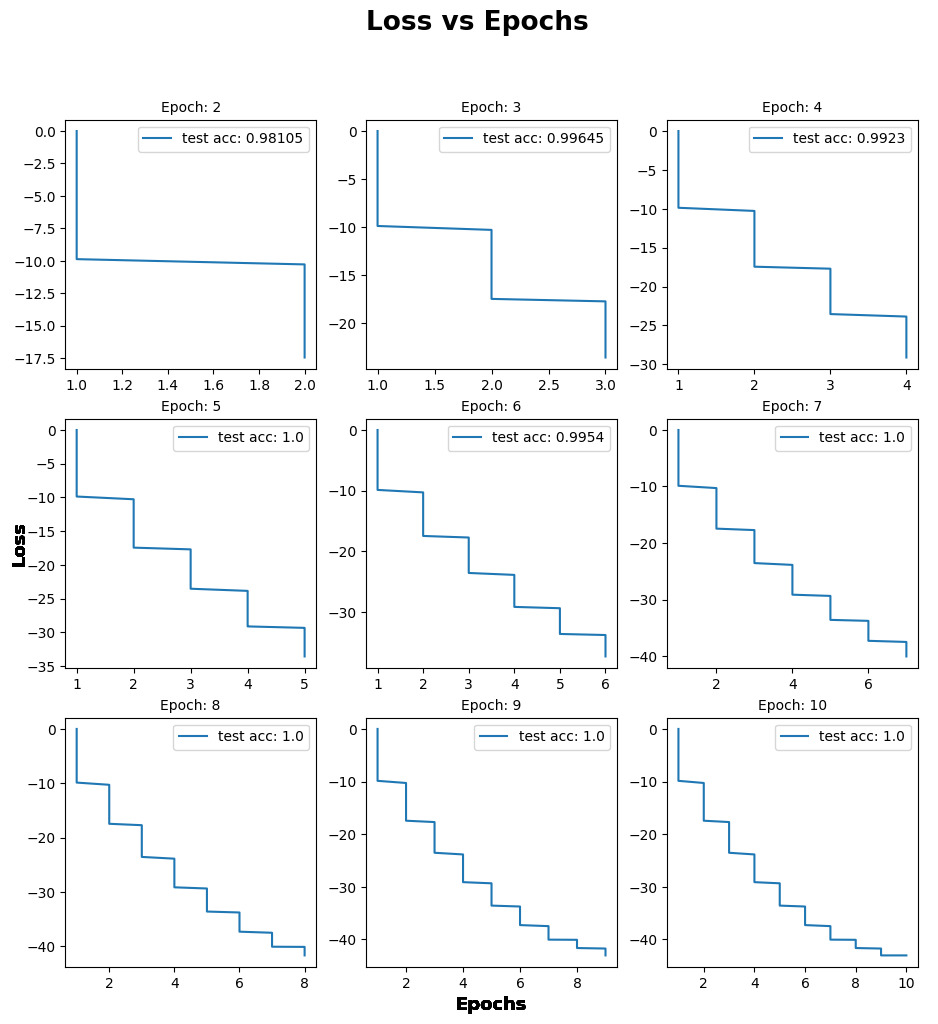
\includegraphics[scale=0.4]{images/Loss.jpeg}
\end{itemize}

\subsection{Explanation for initialization of weights and bias term}
Both the Weights and bias term have been initialised with zero as it was found to be the fastest in converging to a optimised solution.

\section{Answer 6}
\label{A6}
\subsection{Convergence Curve}
Convergence Curve between Time taken and test classificaton Accuracy has been included below.\\
GD stands for Gradient Descent solver method\\
\\
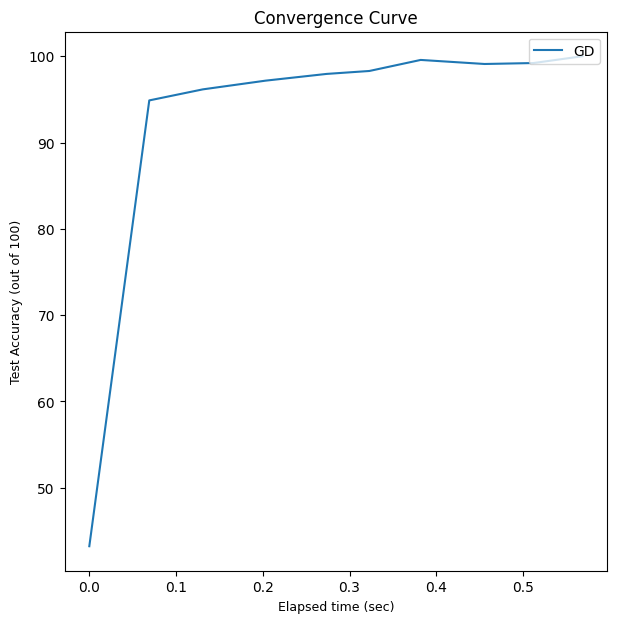
\includegraphics[scale=1]{images/convergence.png}



\section{References}

\medskip

{
\small
[1] https://programmathically.com/understanding-hinge-loss-and-the-svm-cost-function/\\

[2] https://web.cse.iitk.ac.in/users/purushot/courses/ml/2022-23-a/discussion.html
}



\end{document}